\documentclass[../bericht.tex]{subfiles}

\begin{document}

  \begin{appendices}

    \section{Netzteil-Kennlinie}
    \label{sec:netzteil-kennlinie}
      \Cref{fig:netzteil-kennlinie} zeigt die für die Berechnung der Laserschwelle in \cref{subsec:laserschwelle} verwendete Charakterisitk des verwendeten Netzteils.

      \begin{figure}[H]
        \centering
        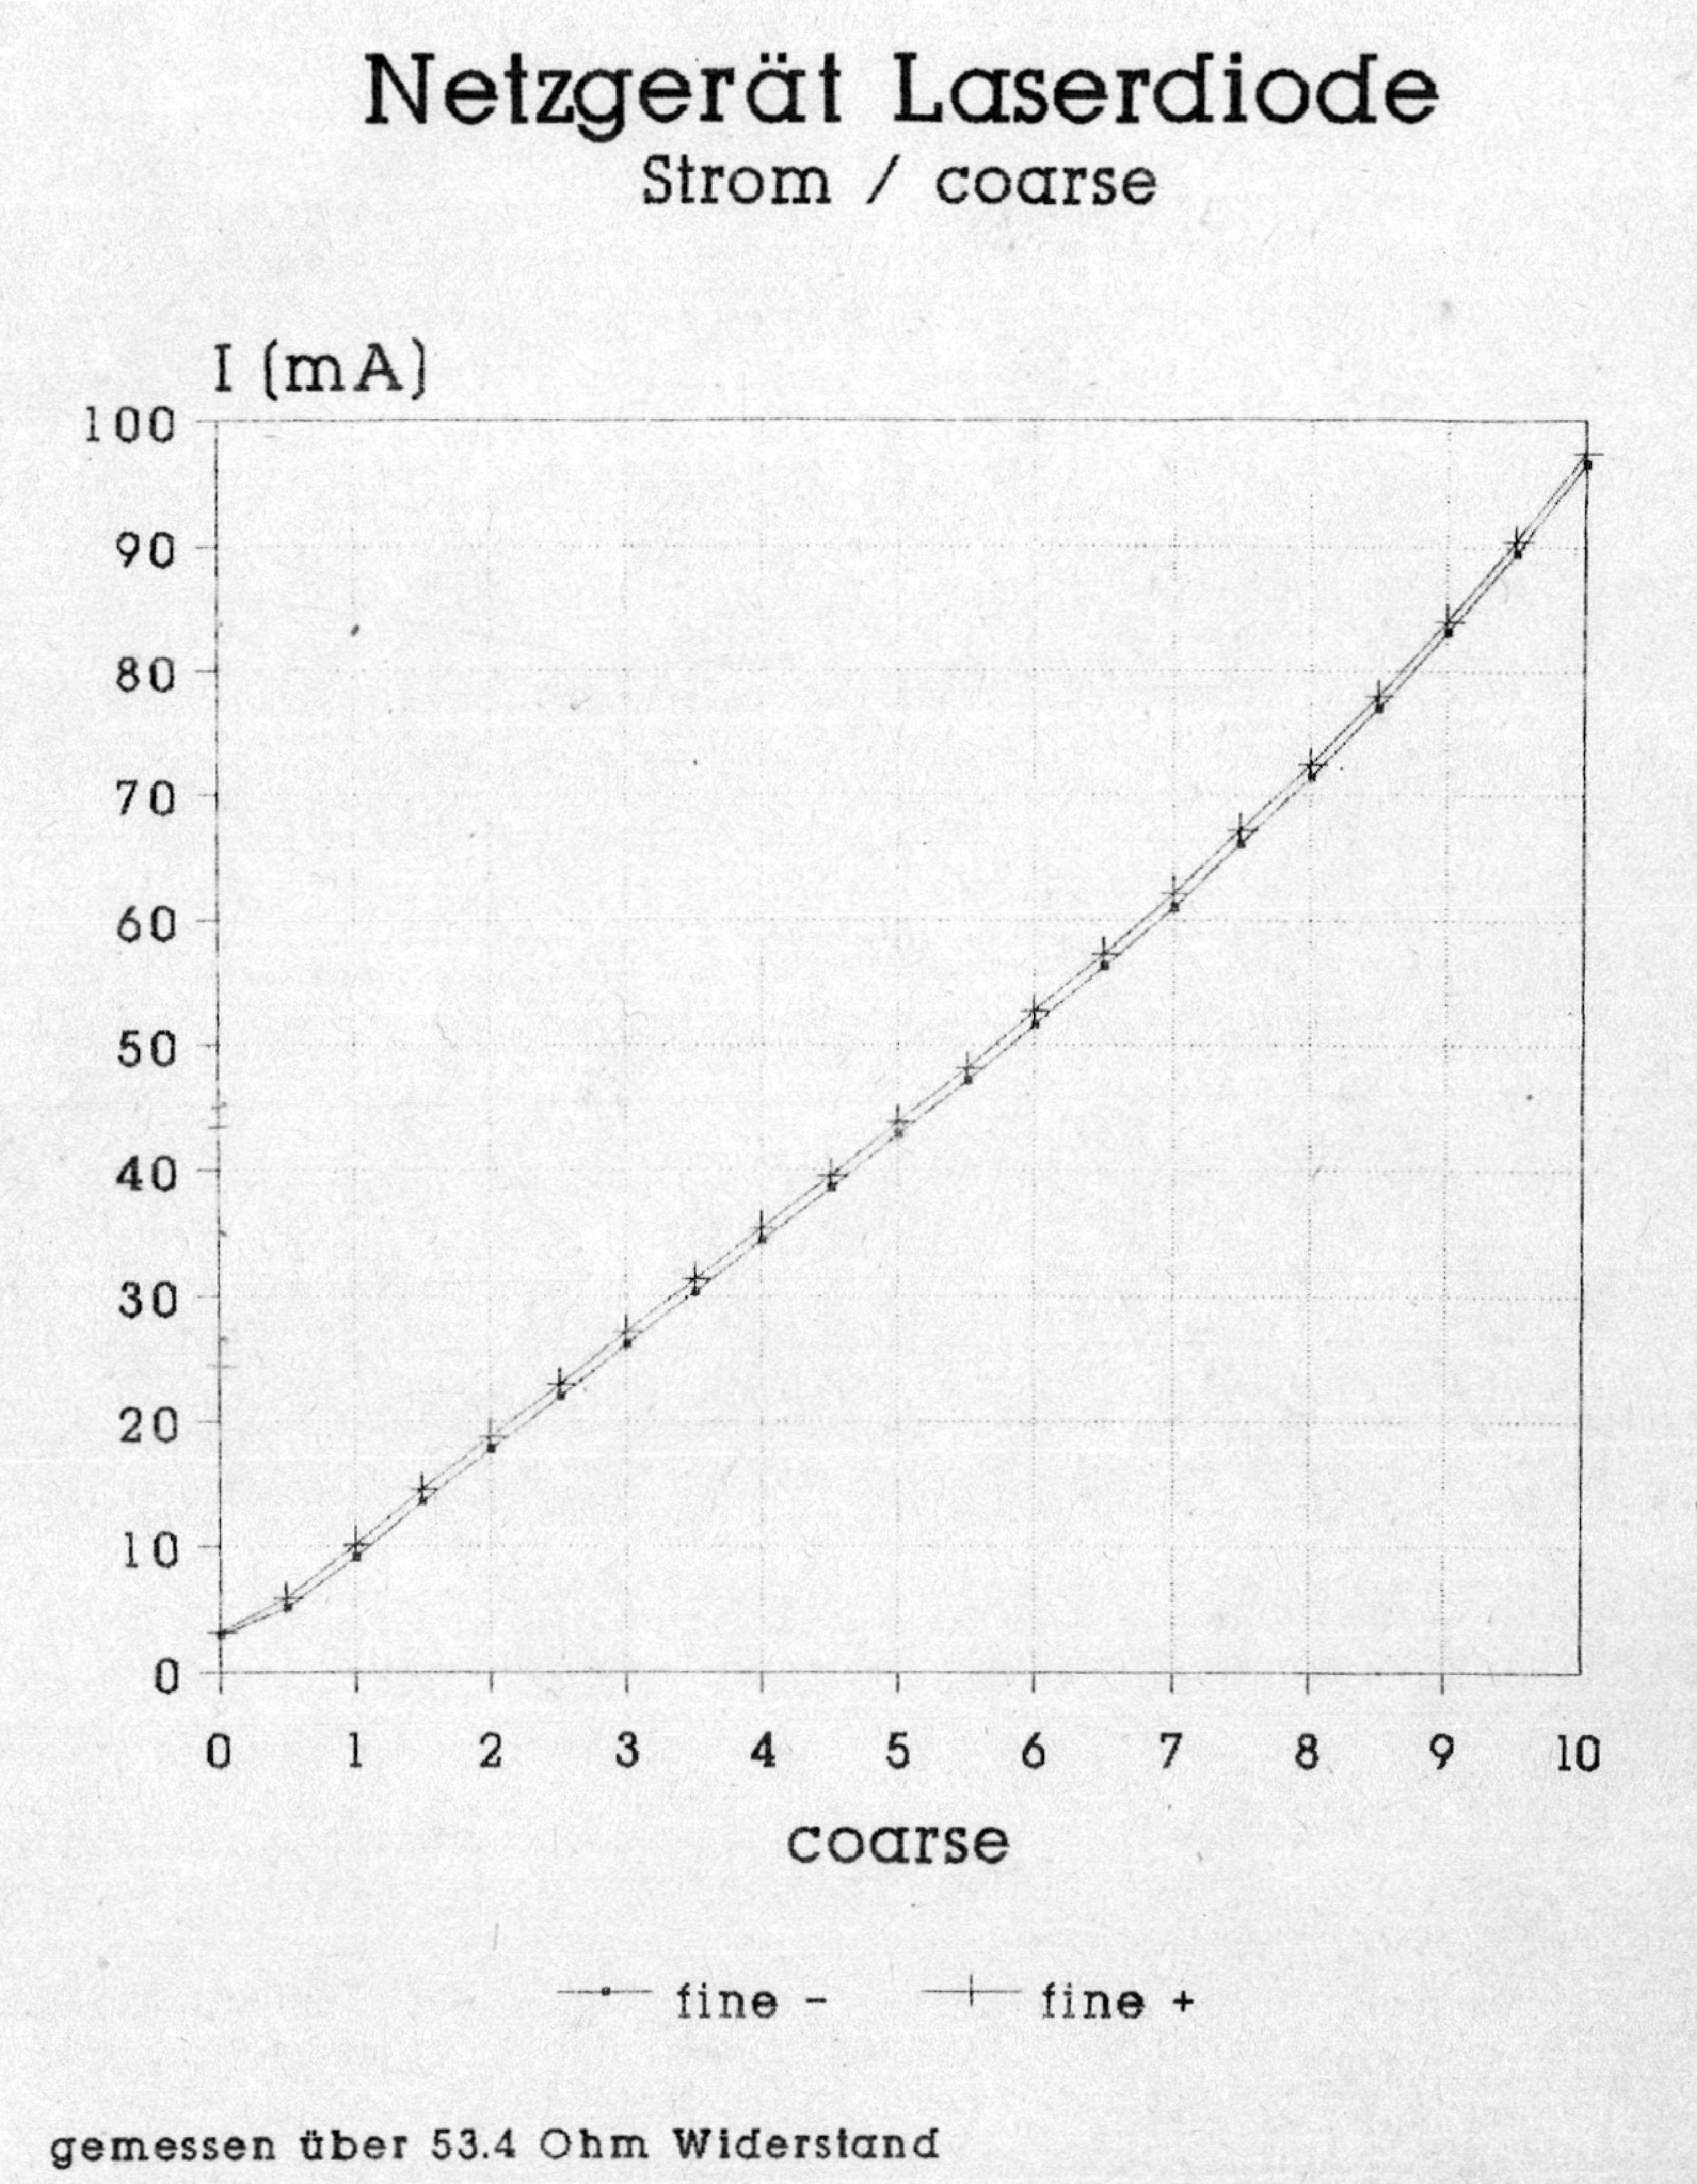
\includegraphics[width=0.85\textwidth]{figures/Stromkennlinie_Laserdiode.pdf}
        \caption{Zusammenhang zwischen dem \textit{Coarse} und der Stromstärke des Netzteils des Diodenlasers.}
        \label{fig:netzteil-kennlinie}
      \end{figure}


    \section{Gau\ss{}fits und Fitparameter}
    \label{sec:gauss-fit-parameter}

      \subsection{Gau\ss{}fit zur Berechnung der Linienbreite des Diodenlasers}
      \label{subsec:fit-linienbreite}

        \begin{table}[ht]
          \caption{Fitparameter des verwendeten fünffachen Gau\ss{}fits \cref{eq:gaussfit} zum fitten der Maxima des ch2 Signals des dopplerfreien Spektrums. Mit $n$ sind die Maxima von links nach rechts numeriert. Die Fitparameter wurden in \cref{subsec:linienbreite-laser} zur Berechnung der Linienbreite des verwendeten Lasers genutzt.}
          \label{tbl:fitparameter-gauss}
          \selectfontsize{10pt}
          \begin{tabu} {X[r]X[r]X[r]X[r]}
            \unitoprule \\
            $n_\mathrm{fit}$ &$t_0$ $[\si{\milli\second}]$  &$V_0$ $[\si{\milli\volt}]$   &$\sigma$ $[\si{\milli\volt}]$  \\
            \tabuphantomline
            \unitoprule \\
            1 &$-5,5875(09)$ &$9,18(28)$ &$-0,0365(13)$ \\
            2 &$-2,8228(14)$ &$6,32(27)$ &$-0,0396(20)$  \\
            3 &$-0,6269(07)$ &$10,88(31)$  &$0,0304(10)$ \\
            4 &$0,9207(09)$  &$10,34(27)$  &$0,0409(12)$ \\
            5 &$3,0375(13)$  &$7,6593(24)$ &$0,0489(18)$ \\
            \unitoprule \\
          \end{tabu}
        \end{table}

        Der zur Auswertung der Linienbreite des verwendeten Diodenlasers genutzter fünffacher Gau\ss{}fit des ch2-Signals des dopplerfreien Spektrums ist gegeben durch
        \begin{equation}
          f(t)=\sum_{n=1}^5 V_0 \cdot \exp \left[ -\left( frac{t-t_0}{\sigma} \right) \right].
          \label{eq:gaussfit}
        \end{equation}
        Die erhaltenen Fitparameter sind in \cref{tbl:fitparameter-gauss} aufgeführt.


      \subsection{Gau\ss{}fit zur Berechnung des Vielfachen des freien Spektralbereichs im dopplerverbreiterten Spektrum}
      \label{subsec:fit-freier-spektralbereich-dopplerverbreitert}

        Für den zweiundzwanzigfachen Gau\ss{}fit des ch2-Signals vom dopplerverbreiterten Spektrum wurde die Formel
        \begin{equation}
          f(t)=\sum_{n=1}^22 V_0 \cdot \exp \left[ -\left( frac{t-t_0}{\sigma} \right) \right]
          \label{eq:gaussfit20}
        \end{equation}
        verwendet und die Fitparameter sind in \cref{tbl:fitparameter-gauss-20} aufgeführt.

        \begin{table}[ht]
          \caption{Fitparameter des verwendeten zweiundzwanzigfachen Gau\ss{}fits \cref{eq:gaussfit20} zum fitten der Maxima des ch2 Signals des dopplerverbreiterten Spektrums. Mit $n$ sind die Maxima von links nach rechts numeriert. Die Fitparameter wurden in \cref{subsec:linienbreite-laser} zur Berechnung des Frequenzabstandes zwischen Grundzustand und angeregtem Zustand verwendet.}
          \label{tbl:fitparameter-gauss-20}
          \selectfontsize{10pt}
          \begin{tabu} {X[r]X[r]X[r]X[r]}
            \unitoprule \\
            $n_\mathrm{fit}$ &$t_0$ $[\si{\milli\second}]$  &$V_0$ $[\si{\milli\volt}]$   &$\sigma$ $[\si{\milli\volt}]$  \\
            \tabuphantomline
            \unitoprule \\
            1 &$-3,7043(08)$ &$12,49(108)$ &$-0,0082(08)$ \\
            2 &$-3,1644(09)$ &$9,89(101)$ &$-0,0090(10)$  \\
            3 &$-2,7978(10)$ &$10,35(121)$  &$0,0078(11)$ \\
            4 &$-2,3645(10)$  &$9,90(104)$  &$0,0083(10)$ \\
            5 &$-1.9057(10)$  &$10,20(093)$ &$0,0081(08)$ \\
            6 &$-1,5614(04)$  &$18,14(391)$ &$0,0076(18)$ \\
            7 &$-1,1199(04)$  &$18,67(202)$ &$0,0083(11)$ \\
            8 &$-0,6989(06)$  &$17,00(186)$ &$0,0077(10)$ \\
            9 &$-0,3602(08)$  &$12,16(536)$ &$0,0072(33)$ \\
            10  &$0,0837(08)$ &$13,62(093)$ &$0,0077(06)$ \\
            11  &$0,4949(19)$ &$5,89(097)$  &$-0,0072(16)$  \\
            12  &$0,8357(10)$ &$9,60(110)$  &$0,0082(11)$ \\
            13  &$1,2580(04)$ &$17,42(258)$ &$-0,0082(15)$  \\
            14  &$1,6617(10)$ &$9,42(116)$  &$0,0086(13)$ \\
            15  &$2,0037(12)$ &$7,58(090)$  &$0,0088(11)$ \\
            16  &$2,4230(07)$ &$15,65(101)$ &$0,0075(06)$ \\
            17  &$2,8549(10)$ &$11,17(102)$ &$0,0073(86)$ \\
            18  &$3,1839(07)$ &$17,20(093)$ &$0,0074(05)$  \\
            19  &$3,6420(08)$ &$12,54(118)$ &$0,0082(09)$ \\
            20  &$4,0392(05)$ &$12,47(275)$ &$0,0081(22)$ \\
            21  &$4,4037(82)$ &$10,94(093)$ &$0,0093(08)$ \\
            22  &$4,8789(05)$ &$12,11(267)$ &$0,0081(22)$ \\
            \unitoprule \\
          \end{tabu}
        \end{table}


      \subsection{Gau\ss{}fit zur Berechnung des Abstandes der Transmissionsminima im dopplerverbreiterten Spektrum}
      \label{subsec:fit-transminima-dopplerverbreitert}

        Für den zweiundzwanzigfachen Gau\ss{}fit des ch2-Signals vom dopplerverbreiterten Spektrum wurde die Formel
        \begin{equation}
          f(t)=\sum_{n=1}^22 V_0 \cdot \exp \left[ -\left( frac{t-t_0}{\sigma} \right) \right]
          \label{eq:gaussfit20}
        \end{equation}
        verwendet und die Fitparameter sind in \cref{tbl:fitparameter-gauss-20} aufgeführt.

        \begin{table}[ht]
          \caption{Fitparameter des verwendeten zweifachen Gau\ss{}fits \cref{eq:gaussfit20} zum fitten der Minima des ch1 Signals des dopplerverbreiterten Spektrums. Mit $n$ sind die Maxima von links nach rechts numeriert. Die Fitparameter wurden in \cref{subsec:linienbreite-laser} zur Berechnung des Frequenzabstandes zwischen Grundzustand und angeregtem Zustand verwendet.}
          \label{tbl:fitparameter-gauss-20}
          \selectfontsize{10pt}
          \begin{tabu} {X[r]X[r]X[r]X[r]}
            \unitoprule \\
            $n_\mathrm{fit}$ &$t_0$ $[\si{\milli\second}]$  &$V_0$ $[\si{\milli\volt}]$   &$\sigma$ $[\si{\milli\volt}]$  \\
            \tabuphantomline
            \unitoprule \\
            1 &$-3,2192(73)$ &$-30,32(085)$ &$-0,321(1)$ \\
            2 &$3,7280(47)$ &$-43,44(092)$ &$-0,271(7)$  \\
            \unitoprule \\
          \end{tabu}
        \end{table}

  \end{appendices}

\end{document}
